\documentclass{article}\usepackage[]{graphicx}\usepackage[]{color}
% maxwidth is the original width if it is less than linewidth
% otherwise use linewidth (to make sure the graphics do not exceed the margin)
\makeatletter
\def\maxwidth{ %
  \ifdim\Gin@nat@width>\linewidth
    \linewidth
  \else
    \Gin@nat@width
  \fi
}
\makeatother

\definecolor{fgcolor}{rgb}{0.345, 0.345, 0.345}
\newcommand{\hlnum}[1]{\textcolor[rgb]{0.686,0.059,0.569}{#1}}%
\newcommand{\hlstr}[1]{\textcolor[rgb]{0.192,0.494,0.8}{#1}}%
\newcommand{\hlcom}[1]{\textcolor[rgb]{0.678,0.584,0.686}{\textit{#1}}}%
\newcommand{\hlopt}[1]{\textcolor[rgb]{0,0,0}{#1}}%
\newcommand{\hlstd}[1]{\textcolor[rgb]{0.345,0.345,0.345}{#1}}%
\newcommand{\hlkwa}[1]{\textcolor[rgb]{0.161,0.373,0.58}{\textbf{#1}}}%
\newcommand{\hlkwb}[1]{\textcolor[rgb]{0.69,0.353,0.396}{#1}}%
\newcommand{\hlkwc}[1]{\textcolor[rgb]{0.333,0.667,0.333}{#1}}%
\newcommand{\hlkwd}[1]{\textcolor[rgb]{0.737,0.353,0.396}{\textbf{#1}}}%
\let\hlipl\hlkwb

\usepackage{framed}
\makeatletter
\newenvironment{kframe}{%
 \def\at@end@of@kframe{}%
 \ifinner\ifhmode%
  \def\at@end@of@kframe{\end{minipage}}%
  \begin{minipage}{\columnwidth}%
 \fi\fi%
 \def\FrameCommand##1{\hskip\@totalleftmargin \hskip-\fboxsep
 \colorbox{shadecolor}{##1}\hskip-\fboxsep
     % There is no \\@totalrightmargin, so:
     \hskip-\linewidth \hskip-\@totalleftmargin \hskip\columnwidth}%
 \MakeFramed {\advance\hsize-\width
   \@totalleftmargin\z@ \linewidth\hsize
   \@setminipage}}%
 {\par\unskip\endMakeFramed%
 \at@end@of@kframe}
\makeatother

\definecolor{shadecolor}{rgb}{.97, .97, .97}
\definecolor{messagecolor}{rgb}{0, 0, 0}
\definecolor{warningcolor}{rgb}{1, 0, 1}
\definecolor{errorcolor}{rgb}{1, 0, 0}
\newenvironment{knitrout}{}{} % an empty environment to be redefined in TeX

\usepackage{alltt}

\title{Flood Frequency Analysis Guide}
\author{Marc Los Huertos}
\IfFileExists{upquote.sty}{\usepackage{upquote}}{}
\begin{document}
\maketitle

\section{Introduction}

\subsection{What is a Flood Frequency Analysis?}

\subsection{Using R to Analyze Flood Frequencies}


\subsubsection{Using Packages to Import Data}

We will use two packages (libraries), `dataRetrieval' and `xts'. To do this, navigage to the Packages tab in the lower right window of Rstudio and click on Install. Type in the names of packages to download.  
\begin{knitrout}
\definecolor{shadecolor}{rgb}{0.969, 0.969, 0.969}\color{fgcolor}\begin{kframe}
\begin{alltt}
\hlcom{### STEP 1}
\hlcom{### Removing previously used scripts from RWater}
\hlcom{### Removing all previously generated datasets and plots }
\hlkwd{cat}\hlstd{(}\hlstr{"\textbackslash{}014"}\hlstd{)}
\end{alltt}
\end{kframe}\begin{kframe}\begin{alltt}
\hlkwd{rm}\hlstd{(}\hlkwc{list} \hlstd{=} \hlkwd{ls}\hlstd{())}
\hlkwd{dev.off}\hlstd{()}
\end{alltt}
\begin{verbatim}
## null device 
##           1
\end{verbatim}
\end{kframe}
\end{knitrout}

\begin{knitrout}
\definecolor{shadecolor}{rgb}{0.969, 0.969, 0.969}\color{fgcolor}\begin{kframe}
\begin{alltt}
\hlcom{### STEP 2}
\hlcom{### Loading two specific packages into RWater  -- not sure what Rwater is...}
\hlkwd{library}\hlstd{(dataRetrieval)}
\hlkwd{library}\hlstd{(xts)}
\end{alltt}


{\ttfamily\noindent\itshape\color{messagecolor}{\#\# Loading required package: zoo}}

{\ttfamily\noindent\itshape\color{messagecolor}{\#\# \\\#\# Attaching package: 'zoo'}}

{\ttfamily\noindent\itshape\color{messagecolor}{\#\# The following objects are masked from 'package:base':\\\#\# \\\#\#\ \ \ \  as.Date, as.Date.numeric}}\end{kframe}
\end{knitrout}


\section{Selecting and Obtaining Gaging Station Data}

\subsection{Finding the Station ID}

I recommend finding a station that has a long record, certianly more than 40 years if you can. 

Using the USGS site, find the station ID and enter below as mysite. The package 

\begin{knitrout}
\definecolor{shadecolor}{rgb}{0.969, 0.969, 0.969}\color{fgcolor}\begin{kframe}
\begin{alltt}
\hlcom{### STEP 3}
\hlcom{### Get the Peak Annual Discharge}
\hlstd{mysite}\hlkwb{<-}\hlstr{'11266500'} \hlcom{# You want to change this code to match your USGS site code. }

\hlstd{annualpeak}\hlkwb{<-}\hlkwd{readNWISpeak}\hlstd{(mysite)}
\hlstd{annualpeak_title} \hlkwb{<-} \hlstr{"Merced River at XXX"}
\end{alltt}
\end{kframe}
\end{knitrout}
\section{Flood Frequency Analysis}

\subsection{Flood Frequency for Entire Record}

First, we'll analyze the data for the entire record -- but you should make sure to do the second part below, where we split the data in half to see if the flood frequencies are consistent. 
\begin{knitrout}
\definecolor{shadecolor}{rgb}{0.969, 0.969, 0.969}\color{fgcolor}\begin{kframe}
\begin{alltt}
\hlcom{### Locate the column of your data set that has the peak discharges}
\hlcom{### Click the 'annualpeak' from your 'Environment' (upper right)}
\hlcom{### You can see that peak discharges are stored in the 6th column (peak_va)}

\hlstd{Q} \hlkwb{<-} \hlstd{annualpeak}\hlopt{$}\hlstd{peak_va}

\hlcom{# Generate plotting positions}
\hlstd{n} \hlkwb{=} \hlkwd{length}\hlstd{(Q)}
\hlstd{r} \hlkwb{=} \hlstd{n} \hlopt{+} \hlnum{1} \hlopt{-} \hlkwd{rank}\hlstd{(Q)}  \hlcom{# highest Q has rank r = 1}
\hlstd{T} \hlkwb{=} \hlstd{(n} \hlopt{+} \hlnum{1}\hlstd{)}\hlopt{/}\hlstd{r}

\hlcom{# Set up x axis tick positions and labels}
\hlstd{Ttick} \hlkwb{=} \hlkwd{c}\hlstd{(}\hlnum{1.001}\hlstd{,}\hlnum{1.01}\hlstd{,}\hlnum{1.1}\hlstd{,}\hlnum{1.5}\hlstd{,}\hlnum{2}\hlstd{,}\hlnum{3}\hlstd{,}\hlnum{4}\hlstd{,}\hlnum{5}\hlstd{,}\hlnum{6}\hlstd{,}\hlnum{7}\hlstd{,}\hlnum{8}\hlstd{,}\hlnum{9}\hlstd{,}\hlnum{10}\hlstd{,}\hlnum{11}\hlstd{,}\hlnum{12}\hlstd{,}
    \hlnum{13}\hlstd{,}\hlnum{14}\hlstd{,}\hlnum{15}\hlstd{,}\hlnum{16}\hlstd{,}\hlnum{17}\hlstd{,}\hlnum{18}\hlstd{,}\hlnum{19}\hlstd{,}\hlnum{20}\hlstd{,}\hlnum{25}\hlstd{,}\hlnum{30}\hlstd{,}\hlnum{35}\hlstd{,}\hlnum{40}\hlstd{,}\hlnum{45}\hlstd{,}\hlnum{50}\hlstd{,}\hlnum{60}\hlstd{,}\hlnum{70}\hlstd{,}
    \hlnum{80}\hlstd{,}\hlnum{90}\hlstd{,}\hlnum{100}\hlstd{)}
\hlstd{xtlab} \hlkwb{=} \hlkwd{c}\hlstd{(}\hlnum{1.001}\hlstd{,}\hlnum{1.01}\hlstd{,}\hlnum{1.1}\hlstd{,}\hlnum{1.5}\hlstd{,}\hlnum{2}\hlstd{,}\hlnum{NA}\hlstd{,}\hlnum{NA}\hlstd{,}\hlnum{5}\hlstd{,}\hlnum{NA}\hlstd{,}\hlnum{NA}\hlstd{,}\hlnum{NA}\hlstd{,}\hlnum{NA}\hlstd{,}\hlnum{10}\hlstd{,}
    \hlnum{NA}\hlstd{,}\hlnum{NA}\hlstd{,}\hlnum{NA}\hlstd{,}\hlnum{NA}\hlstd{,}\hlnum{15}\hlstd{,}\hlnum{NA}\hlstd{,}\hlnum{NA}\hlstd{,}\hlnum{NA}\hlstd{,}\hlnum{NA}\hlstd{,}\hlnum{20}\hlstd{,}\hlnum{NA}\hlstd{,}\hlnum{30}\hlstd{,}\hlnum{NA}\hlstd{,}\hlnum{NA}\hlstd{,}\hlnum{NA}\hlstd{,}\hlnum{50}\hlstd{,}\hlnum{NA}\hlstd{,}\hlnum{NA}\hlstd{,}
    \hlnum{NA}\hlstd{,}\hlnum{NA}\hlstd{,}\hlnum{100}\hlstd{)}
\hlstd{y} \hlkwb{=} \hlopt{-}\hlkwd{log}\hlstd{(}\hlopt{-}\hlkwd{log}\hlstd{(}\hlnum{1} \hlopt{-} \hlnum{1}\hlopt{/}\hlstd{T))}
\hlstd{ytick} \hlkwb{=} \hlopt{-}\hlkwd{log}\hlstd{(}\hlopt{-}\hlkwd{log}\hlstd{(}\hlnum{1} \hlopt{-} \hlnum{1}\hlopt{/}\hlstd{Ttick))}
\hlstd{xmin} \hlkwb{=} \hlkwd{min}\hlstd{(}\hlkwd{min}\hlstd{(y),}\hlkwd{min}\hlstd{(ytick))}
\hlstd{xmax} \hlkwb{=} \hlkwd{max}\hlstd{(ytick)}

\hlcom{# Fit a line by method of moments, along with 95% confidence intervals}
\hlstd{KTtick} \hlkwb{=} \hlopt{-}\hlstd{(}\hlkwd{sqrt}\hlstd{(}\hlnum{6}\hlstd{)}\hlopt{/}\hlstd{pi)}\hlopt{*}\hlstd{(}\hlnum{0.5772} \hlopt{+} \hlkwd{log}\hlstd{(}\hlkwd{log}\hlstd{(Ttick}\hlopt{/}\hlstd{(Ttick}\hlopt{-}\hlnum{1}\hlstd{))))}
\hlstd{QTtick} \hlkwb{=} \hlkwd{mean}\hlstd{(Q)} \hlopt{+} \hlstd{KTtick}\hlopt{*}\hlkwd{sd}\hlstd{(Q)}
\hlstd{nQ} \hlkwb{=} \hlkwd{length}\hlstd{(Q)}
\hlstd{se} \hlkwb{=} \hlstd{(}\hlkwd{sd}\hlstd{(Q)}\hlopt{*}\hlkwd{sqrt}\hlstd{((}\hlnum{1}\hlopt{+}\hlnum{1.14}\hlopt{*}\hlstd{KTtick} \hlopt{+} \hlnum{1.1}\hlopt{*}\hlstd{KTtick}\hlopt{^}\hlnum{2}\hlstd{)))}\hlopt{/}\hlkwd{sqrt}\hlstd{(nQ)}
\hlstd{LB} \hlkwb{=} \hlstd{QTtick} \hlopt{-} \hlkwd{qt}\hlstd{(}\hlnum{0.975}\hlstd{, nQ} \hlopt{-} \hlnum{1}\hlstd{)}\hlopt{*}\hlstd{se}
\hlstd{UB} \hlkwb{=} \hlstd{QTtick} \hlopt{+} \hlkwd{qt}\hlstd{(}\hlnum{0.975}\hlstd{, nQ} \hlopt{-} \hlnum{1}\hlstd{)}\hlopt{*}\hlstd{se}
\hlstd{max} \hlkwb{=} \hlkwd{max}\hlstd{(UB)}
\hlstd{Qmax} \hlkwb{=} \hlkwd{max}\hlstd{(QTtick)}

\hlcom{# Plot peak flow series with Gumbel axis}
\hlkwd{plot}\hlstd{(y, Q,}
     \hlkwc{ylab} \hlstd{=} \hlkwd{expression}\hlstd{(} \hlstr{"Annual Peak Flow (cfs)"} \hlstd{) ,}
     \hlkwc{xaxt} \hlstd{=} \hlstr{"n"}\hlstd{,} \hlkwc{xlab} \hlstd{=} \hlstr{"Return Period, T (year)"}\hlstd{,}
     \hlkwc{ylim} \hlstd{=} \hlkwd{c}\hlstd{(}\hlnum{0}\hlstd{, Qmax),}
     \hlkwc{xlim} \hlstd{=} \hlkwd{c}\hlstd{(xmin, xmax),}
     \hlkwc{pch} \hlstd{=} \hlnum{21}\hlstd{,} \hlkwc{bg} \hlstd{=} \hlstr{"red"}\hlstd{,}
     \hlkwc{main} \hlstd{= annualpeak_title}
\hlstd{)}
\hlkwd{par}\hlstd{(}\hlkwc{cex} \hlstd{=} \hlnum{0.65}\hlstd{)}
\hlkwd{axis}\hlstd{(}\hlnum{1}\hlstd{,} \hlkwc{at} \hlstd{= ytick,} \hlkwc{labels} \hlstd{=} \hlkwd{as.character}\hlstd{(xtlab))}

\hlcom{# Add fitted line and confidence limits}
\hlkwd{lines}\hlstd{(ytick, QTtick,} \hlkwc{col} \hlstd{=} \hlstr{"black"}\hlstd{,} \hlkwc{lty}\hlstd{=}\hlnum{1}\hlstd{,} \hlkwc{lwd}\hlstd{=}\hlnum{2}\hlstd{)}
\hlkwd{lines}\hlstd{(ytick, LB,} \hlkwc{col} \hlstd{=} \hlstr{"blue"}\hlstd{,} \hlkwc{lty} \hlstd{=} \hlnum{1}\hlstd{,} \hlkwc{lwd}\hlstd{=}\hlnum{1.5}\hlstd{)}
\hlkwd{lines}\hlstd{(ytick, UB,} \hlkwc{col} \hlstd{=} \hlstr{"red"}\hlstd{,} \hlkwc{lty} \hlstd{=} \hlnum{1}\hlstd{,} \hlkwc{lwd}\hlstd{=}\hlnum{1.5}\hlstd{)}
\hlcom{# Draw grid lines}
\hlkwd{abline}\hlstd{(}\hlkwc{v} \hlstd{= ytick,} \hlkwc{lty} \hlstd{=} \hlnum{3}\hlstd{,} \hlkwc{col}\hlstd{=}\hlstr{"light gray"}\hlstd{)}
\hlkwd{abline}\hlstd{(}\hlkwc{h} \hlstd{=} \hlkwd{seq}\hlstd{(}\hlnum{500}\hlstd{,} \hlkwd{floor}\hlstd{(Qmax),} \hlnum{500}\hlstd{),} \hlkwc{lty} \hlstd{=} \hlnum{3}\hlstd{,}\hlkwc{col}\hlstd{=}\hlstr{"light gray"}\hlstd{)}
\end{alltt}
\end{kframe}
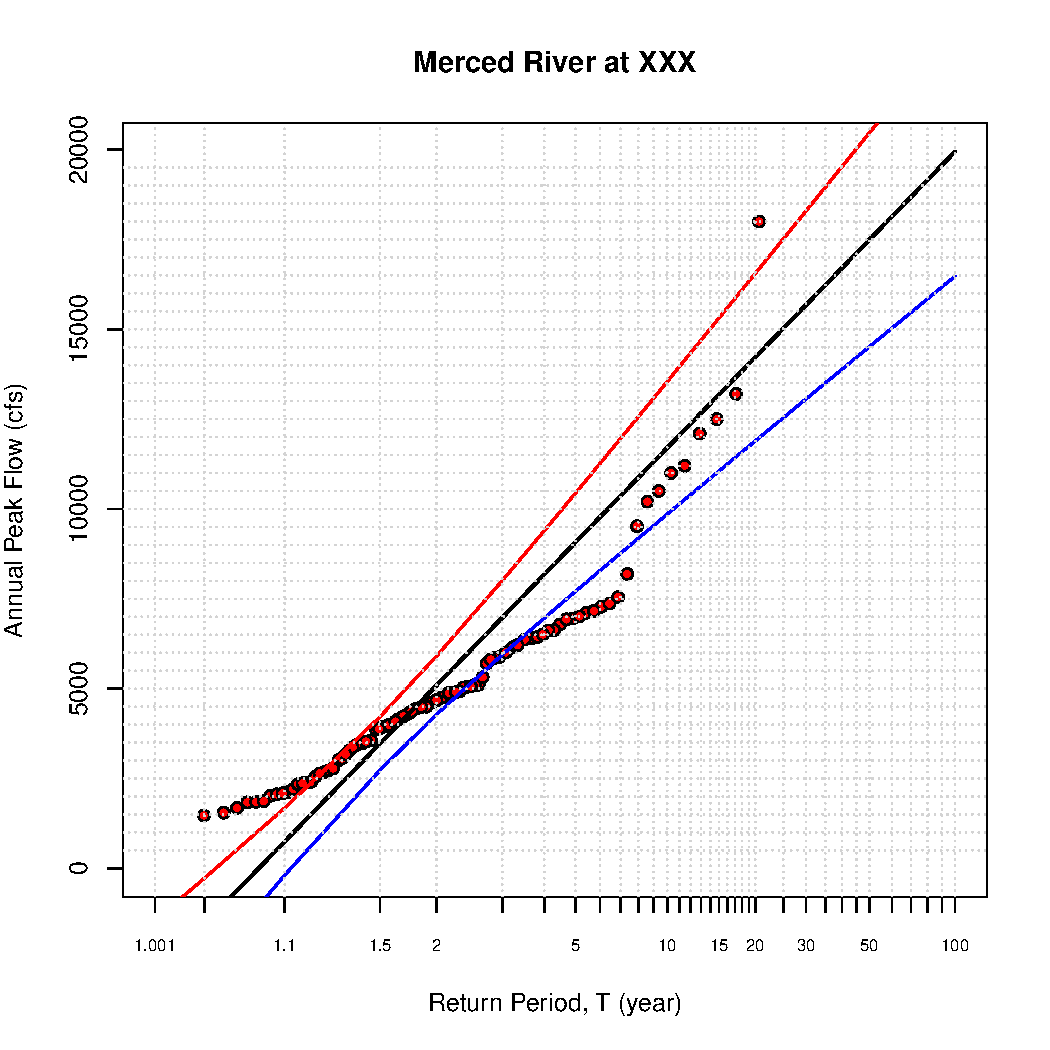
\includegraphics[width=\maxwidth]{figure/unnamed-chunk-4-1} 
\begin{kframe}\begin{alltt}
\hlkwd{par}\hlstd{(}\hlkwc{cex} \hlstd{=} \hlnum{1}\hlstd{)}
\end{alltt}
\end{kframe}
\end{knitrout}

\section{Are Flood Frequencies Stationary?}

\subsection{Testing if the data are consistent over time}

Look at the data and evaluate how to split the data in half -- then we can see if the estimate for flood frequency has changed. 

Remember, in California, the water year actually starts on the 1st of October each year. In the example, I have below, I have define the dates, name of the station and dates for the graphic labels in this section too. 

\begin{knitrout}
\definecolor{shadecolor}{rgb}{0.969, 0.969, 0.969}\color{fgcolor}\begin{kframe}
\begin{alltt}
\hlcom{### STEP 4}
\hlcom{### Split the downloaded data into two 20 year periods}
\hlcom{### Water year in CA, begins Oct 1 each year.}

\hlstd{period1}\hlkwb{<-}\hlkwd{subset}\hlstd{(annualpeak,}
               \hlstd{peak_dt}\hlopt{>=}\hlstr{"1980-10-01"}
               \hlopt{&}\hlstd{peak_dt}\hlopt{<=}\hlstr{"1999-09-30"}\hlstd{)}
\hlstd{period1_title} \hlkwb{=} \hlstr{"Merced River at XXX, (1980-1999)"}
\hlstd{period2}\hlkwb{<-}\hlkwd{subset}\hlstd{(annualpeak,}
                \hlstd{peak_dt}\hlopt{>=}\hlstr{"1999-10-01"}
                \hlopt{&}\hlstd{peak_dt}\hlopt{<=}\hlstr{"2019-09-30"}\hlstd{)}
\hlstd{period2_title} \hlkwb{=} \hlstr{"Merced River at XXX, (2000-2019)"}
\hlstd{ymax} \hlkwb{=} \hlkwd{round}\hlstd{(}\hlkwd{max}\hlstd{(annualpeak}\hlopt{$}\hlstd{peak_va,} \hlkwc{na.rm}\hlstd{=T)}\hlopt{*}\hlnum{1.1}\hlstd{,} \hlopt{-}\hlnum{3}\hlstd{)}
\end{alltt}
\end{kframe}
\end{knitrout}


\begin{knitrout}
\definecolor{shadecolor}{rgb}{0.969, 0.969, 0.969}\color{fgcolor}\begin{kframe}
\begin{alltt}
\hlcom{### STEP 5}
\end{alltt}
\end{kframe}
\end{knitrout}

\section{Flood Frequency Analysis for Two Periods}
\begin{knitrout}
\definecolor{shadecolor}{rgb}{0.969, 0.969, 0.969}\color{fgcolor}\begin{kframe}
\begin{alltt}
\hlcom{### STEP 5}
\hlcom{### Perform Flood Freqency Analysis }
\hlcom{### Locate the column of your data set that has the peak discharges}
\hlcom{### Click the 'period1' from your 'Environment' (upper right)}
\hlcom{### You can see that peak discharges are stored in the 6th column (peak_va)}

\hlstd{Q} \hlkwb{<-} \hlstd{period1}\hlopt{$}\hlstd{peak_va}

\hlcom{#Generate plotting positions}
\hlstd{n} \hlkwb{=} \hlkwd{length}\hlstd{(Q)}
\hlstd{r} \hlkwb{=} \hlstd{n} \hlopt{+} \hlnum{1} \hlopt{-} \hlkwd{rank}\hlstd{(Q)}  \hlcom{# highest Q has rank r = 1}
\hlstd{T} \hlkwb{=} \hlstd{(n} \hlopt{+} \hlnum{1}\hlstd{)}\hlopt{/}\hlstd{r}

\hlcom{# Set up x axis tick positions and labels}
\hlstd{Ttick} \hlkwb{=} \hlkwd{c}\hlstd{(}\hlnum{1.001}\hlstd{,}\hlnum{1.01}\hlstd{,}\hlnum{1.1}\hlstd{,}\hlnum{1.5}\hlstd{,}\hlnum{2}\hlstd{,}\hlnum{3}\hlstd{,}\hlnum{4}\hlstd{,}\hlnum{5}\hlstd{,}\hlnum{6}\hlstd{,}\hlnum{7}\hlstd{,}\hlnum{8}\hlstd{,}\hlnum{9}\hlstd{,}\hlnum{10}\hlstd{,}\hlnum{11}\hlstd{,}\hlnum{12}\hlstd{,}
    \hlnum{13}\hlstd{,}\hlnum{14}\hlstd{,}\hlnum{15}\hlstd{,}\hlnum{16}\hlstd{,}\hlnum{17}\hlstd{,}\hlnum{18}\hlstd{,}\hlnum{19}\hlstd{,}\hlnum{20}\hlstd{,}\hlnum{25}\hlstd{,}\hlnum{30}\hlstd{,}\hlnum{35}\hlstd{,}\hlnum{40}\hlstd{,}\hlnum{45}\hlstd{,}\hlnum{50}\hlstd{,}\hlnum{60}\hlstd{,}\hlnum{70}\hlstd{,}
    \hlnum{80}\hlstd{,}\hlnum{90}\hlstd{,}\hlnum{100}\hlstd{)}
\hlstd{xtlab} \hlkwb{=} \hlkwd{c}\hlstd{(}\hlnum{1.001}\hlstd{,}\hlnum{1.01}\hlstd{,}\hlnum{1.1}\hlstd{,}\hlnum{1.5}\hlstd{,}\hlnum{2}\hlstd{,}\hlnum{NA}\hlstd{,}\hlnum{NA}\hlstd{,}\hlnum{5}\hlstd{,}\hlnum{NA}\hlstd{,}\hlnum{NA}\hlstd{,}\hlnum{NA}\hlstd{,}\hlnum{NA}\hlstd{,}\hlnum{10}\hlstd{,}
    \hlnum{NA}\hlstd{,}\hlnum{NA}\hlstd{,}\hlnum{NA}\hlstd{,}\hlnum{NA}\hlstd{,}\hlnum{15}\hlstd{,}\hlnum{NA}\hlstd{,}\hlnum{NA}\hlstd{,}\hlnum{NA}\hlstd{,}\hlnum{NA}\hlstd{,}\hlnum{20}\hlstd{,}\hlnum{NA}\hlstd{,}\hlnum{30}\hlstd{,}\hlnum{NA}\hlstd{,}\hlnum{NA}\hlstd{,}\hlnum{NA}\hlstd{,}\hlnum{50}\hlstd{,}\hlnum{NA}\hlstd{,}\hlnum{NA}\hlstd{,}
    \hlnum{NA}\hlstd{,}\hlnum{NA}\hlstd{,}\hlnum{100}\hlstd{)}
\hlstd{y} \hlkwb{=} \hlopt{-}\hlkwd{log}\hlstd{(}\hlopt{-}\hlkwd{log}\hlstd{(}\hlnum{1} \hlopt{-} \hlnum{1}\hlopt{/}\hlstd{T))}
\hlstd{ytick} \hlkwb{=} \hlopt{-}\hlkwd{log}\hlstd{(}\hlopt{-}\hlkwd{log}\hlstd{(}\hlnum{1} \hlopt{-} \hlnum{1}\hlopt{/}\hlstd{Ttick))}
\hlstd{xmin} \hlkwb{=} \hlkwd{min}\hlstd{(}\hlkwd{min}\hlstd{(y),}\hlkwd{min}\hlstd{(ytick))}
\hlstd{xmax} \hlkwb{=} \hlkwd{max}\hlstd{(ytick)}

\hlcom{# Fit a line by method of moments, along with 95% confidence intervals}
\hlstd{KTtick} \hlkwb{=} \hlopt{-}\hlstd{(}\hlkwd{sqrt}\hlstd{(}\hlnum{6}\hlstd{)}\hlopt{/}\hlstd{pi)}\hlopt{*}\hlstd{(}\hlnum{0.5772} \hlopt{+} \hlkwd{log}\hlstd{(}\hlkwd{log}\hlstd{(Ttick}\hlopt{/}\hlstd{(Ttick}\hlopt{-}\hlnum{1}\hlstd{))))}
\hlstd{QTtick} \hlkwb{=} \hlkwd{mean}\hlstd{(Q)} \hlopt{+} \hlstd{KTtick}\hlopt{*}\hlkwd{sd}\hlstd{(Q)}
\hlstd{nQ} \hlkwb{=} \hlkwd{length}\hlstd{(Q)}
\hlstd{se} \hlkwb{=} \hlstd{(}\hlkwd{sd}\hlstd{(Q)}\hlopt{*}\hlkwd{sqrt}\hlstd{((}\hlnum{1}\hlopt{+}\hlnum{1.14}\hlopt{*}\hlstd{KTtick} \hlopt{+} \hlnum{1.1}\hlopt{*}\hlstd{KTtick}\hlopt{^}\hlnum{2}\hlstd{)))}\hlopt{/}\hlkwd{sqrt}\hlstd{(nQ)}
\hlstd{LB} \hlkwb{=} \hlstd{QTtick} \hlopt{-} \hlkwd{qt}\hlstd{(}\hlnum{0.975}\hlstd{, nQ} \hlopt{-} \hlnum{1}\hlstd{)}\hlopt{*}\hlstd{se}
\hlstd{UB} \hlkwb{=} \hlstd{QTtick} \hlopt{+} \hlkwd{qt}\hlstd{(}\hlnum{0.975}\hlstd{, nQ} \hlopt{-} \hlnum{1}\hlstd{)}\hlopt{*}\hlstd{se}
\hlstd{max} \hlkwb{=} \hlkwd{max}\hlstd{(UB)}
\hlstd{Qmax} \hlkwb{=} \hlkwd{max}\hlstd{(QTtick)}

\hlcom{### Split the plot window in two columns}
\hlkwd{par}\hlstd{(}\hlkwc{mfrow}\hlstd{=}\hlkwd{c}\hlstd{(}\hlnum{1}\hlstd{,}\hlnum{2}\hlstd{))}

\hlcom{# Plot peak flow series with Gumbel axis}
\hlkwd{plot}\hlstd{(y, Q,}
     \hlkwc{ylab} \hlstd{=} \hlkwd{expression}\hlstd{(} \hlstr{"Annual Peak Flow (cfs)"} \hlstd{) ,}
     \hlkwc{xaxt} \hlstd{=} \hlstr{"n"}\hlstd{,} \hlkwc{xlab} \hlstd{=} \hlstr{"Return Period, T (year)"}\hlstd{,}
     \hlkwc{ylim} \hlstd{=} \hlkwd{c}\hlstd{(}\hlnum{0}\hlstd{, ymax),}
     \hlkwc{xlim} \hlstd{=} \hlkwd{c}\hlstd{(xmin, xmax),}
     \hlkwc{pch} \hlstd{=} \hlnum{21}\hlstd{,} \hlkwc{bg} \hlstd{=} \hlstr{"red"}\hlstd{,}
     \hlkwc{main} \hlstd{= period1_title}
\hlstd{)}
\hlkwd{par}\hlstd{(}\hlkwc{cex} \hlstd{=} \hlnum{0.65}\hlstd{)}
\hlkwd{axis}\hlstd{(}\hlnum{1}\hlstd{,} \hlkwc{at} \hlstd{= ytick,} \hlkwc{labels} \hlstd{=} \hlkwd{as.character}\hlstd{(xtlab))}

\hlcom{# Add fitted line and confidence limits}
\hlkwd{lines}\hlstd{(ytick, QTtick,} \hlkwc{col} \hlstd{=} \hlstr{"black"}\hlstd{,} \hlkwc{lty}\hlstd{=}\hlnum{1}\hlstd{,} \hlkwc{lwd}\hlstd{=}\hlnum{2}\hlstd{)}
\hlkwd{lines}\hlstd{(ytick, LB,} \hlkwc{col} \hlstd{=} \hlstr{"blue"}\hlstd{,} \hlkwc{lty} \hlstd{=} \hlnum{1}\hlstd{,} \hlkwc{lwd}\hlstd{=}\hlnum{1.5}\hlstd{)}
\hlkwd{lines}\hlstd{(ytick, UB,} \hlkwc{col} \hlstd{=} \hlstr{"red"}\hlstd{,} \hlkwc{lty} \hlstd{=} \hlnum{1}\hlstd{,} \hlkwc{lwd}\hlstd{=}\hlnum{1.5}\hlstd{)}

\hlcom{# Draw grid lines}
\hlkwd{abline}\hlstd{(}\hlkwc{v} \hlstd{= ytick,} \hlkwc{lty} \hlstd{=} \hlnum{3}\hlstd{,} \hlkwc{col}\hlstd{=}\hlstr{"light gray"}\hlstd{)}
\hlkwd{abline}\hlstd{(}\hlkwc{h} \hlstd{=} \hlkwd{seq}\hlstd{(}\hlnum{500}\hlstd{,} \hlkwd{floor}\hlstd{(Qmax),} \hlnum{500}\hlstd{),} \hlkwc{lty} \hlstd{=} \hlnum{3}\hlstd{,}\hlkwc{col}\hlstd{=}\hlstr{"light gray"}\hlstd{)}
\hlkwd{par}\hlstd{(}\hlkwc{cex} \hlstd{=} \hlnum{1}\hlstd{)}


\hlcom{### Perform Flood Freqency Analysis for the second time period}

\hlstd{Q} \hlkwb{=} \hlstd{period2}\hlopt{$}\hlstd{peak_va}

\hlcom{#Generate plotting positions}
\hlstd{n} \hlkwb{=} \hlkwd{length}\hlstd{(Q)}
\hlstd{r} \hlkwb{=} \hlstd{n} \hlopt{+} \hlnum{1} \hlopt{-} \hlkwd{rank}\hlstd{(Q)}  \hlcom{# highest Q has rank r = 1}
\hlstd{T} \hlkwb{=} \hlstd{(n} \hlopt{+} \hlnum{1}\hlstd{)}\hlopt{/}\hlstd{r}

\hlcom{# Set up x axis tick positions and labels}
\hlcom{#Ttick = c(1.001,1.01,1.1,1.5,2,3,4,5,6,7,8,9,10,11,12,13,14,15,16,17,18,19,20,25,30,35,40,45,50,60,70,80,90,100)}
\hlcom{#xtlab = c(1.001,1.01,1.1,1.5,2,NA,NA,5,NA,NA,NA,NA,10,NA,NA,NA,NA,15,NA,NA,NA,NA,20,NA,30,NA,NA,NA,50,NA,NA,NA,NA,100)}
\hlstd{y} \hlkwb{=} \hlopt{-}\hlkwd{log}\hlstd{(}\hlopt{-}\hlkwd{log}\hlstd{(}\hlnum{1} \hlopt{-} \hlnum{1}\hlopt{/}\hlstd{T))}
\hlstd{ytick} \hlkwb{=} \hlopt{-}\hlkwd{log}\hlstd{(}\hlopt{-}\hlkwd{log}\hlstd{(}\hlnum{1} \hlopt{-} \hlnum{1}\hlopt{/}\hlstd{Ttick))}
\hlstd{xmin} \hlkwb{=} \hlkwd{min}\hlstd{(}\hlkwd{min}\hlstd{(y),}\hlkwd{min}\hlstd{(ytick))}
\hlstd{xmax} \hlkwb{=} \hlkwd{max}\hlstd{(ytick)}

\hlcom{# Fit a line by method of moments, along with 95% confidence intervals}
\hlstd{KTtick} \hlkwb{=} \hlopt{-}\hlstd{(}\hlkwd{sqrt}\hlstd{(}\hlnum{6}\hlstd{)}\hlopt{/}\hlstd{pi)}\hlopt{*}\hlstd{(}\hlnum{0.5772} \hlopt{+} \hlkwd{log}\hlstd{(}\hlkwd{log}\hlstd{(Ttick}\hlopt{/}\hlstd{(Ttick}\hlopt{-}\hlnum{1}\hlstd{))))}
\hlstd{QTtick} \hlkwb{=} \hlkwd{mean}\hlstd{(Q)} \hlopt{+} \hlstd{KTtick}\hlopt{*}\hlkwd{sd}\hlstd{(Q)}
\hlstd{nQ} \hlkwb{=} \hlkwd{length}\hlstd{(Q)}
\hlstd{se} \hlkwb{=} \hlstd{(}\hlkwd{sd}\hlstd{(Q)}\hlopt{*}\hlkwd{sqrt}\hlstd{((}\hlnum{1}\hlopt{+}\hlnum{1.14}\hlopt{*}\hlstd{KTtick} \hlopt{+} \hlnum{1.1}\hlopt{*}\hlstd{KTtick}\hlopt{^}\hlnum{2}\hlstd{)))}\hlopt{/}\hlkwd{sqrt}\hlstd{(nQ)}
\hlstd{LB} \hlkwb{=} \hlstd{QTtick} \hlopt{-} \hlkwd{qt}\hlstd{(}\hlnum{0.975}\hlstd{, nQ} \hlopt{-} \hlnum{1}\hlstd{)}\hlopt{*}\hlstd{se}
\hlstd{UB} \hlkwb{=} \hlstd{QTtick} \hlopt{+} \hlkwd{qt}\hlstd{(}\hlnum{0.975}\hlstd{, nQ} \hlopt{-} \hlnum{1}\hlstd{)}\hlopt{*}\hlstd{se}
\hlstd{max} \hlkwb{=} \hlkwd{max}\hlstd{(UB)}
\hlstd{Qmax} \hlkwb{=} \hlkwd{max}\hlstd{(QTtick)}

\hlcom{# Plot peak flow series with Gumbel axis}
\hlkwd{plot}\hlstd{(y, Q,}
     \hlkwc{ylab} \hlstd{=} \hlkwd{expression}\hlstd{(} \hlstr{"Annual Peak Flow (cfs)"} \hlstd{) ,}
     \hlkwc{xaxt} \hlstd{=} \hlstr{"n"}\hlstd{,} \hlkwc{xlab} \hlstd{=} \hlstr{"Return Period, T (year)"}\hlstd{,}
     \hlkwc{ylim} \hlstd{=} \hlkwd{c}\hlstd{(}\hlnum{0}\hlstd{, ymax),}
     \hlkwc{xlim} \hlstd{=} \hlkwd{c}\hlstd{(xmin, xmax),}
     \hlkwc{pch} \hlstd{=} \hlnum{21}\hlstd{,} \hlkwc{bg} \hlstd{=} \hlstr{"red"}\hlstd{,}
     \hlkwc{main} \hlstd{= period2_title}
\hlstd{)}
\hlkwd{par}\hlstd{(}\hlkwc{cex} \hlstd{=} \hlnum{0.65}\hlstd{)}
\hlkwd{axis}\hlstd{(}\hlnum{1}\hlstd{,} \hlkwc{at} \hlstd{= ytick,} \hlkwc{labels} \hlstd{=} \hlkwd{as.character}\hlstd{(xtlab))}

\hlcom{# Add fitted line and confidence limits}
\hlkwd{lines}\hlstd{(ytick, QTtick,} \hlkwc{col} \hlstd{=} \hlstr{"black"}\hlstd{,} \hlkwc{lty}\hlstd{=}\hlnum{1}\hlstd{,} \hlkwc{lwd}\hlstd{=}\hlnum{2}\hlstd{)}
\hlkwd{lines}\hlstd{(ytick, LB,} \hlkwc{col} \hlstd{=} \hlstr{"blue"}\hlstd{,} \hlkwc{lty} \hlstd{=} \hlnum{1}\hlstd{,} \hlkwc{lwd}\hlstd{=}\hlnum{1.5}\hlstd{)}
\hlkwd{lines}\hlstd{(ytick, UB,} \hlkwc{col} \hlstd{=} \hlstr{"red"}\hlstd{,} \hlkwc{lty} \hlstd{=} \hlnum{1}\hlstd{,} \hlkwc{lwd}\hlstd{=}\hlnum{1.5}\hlstd{)}

\hlcom{# Draw grid lines}
\hlkwd{abline}\hlstd{(}\hlkwc{v} \hlstd{= ytick,} \hlkwc{lty} \hlstd{=} \hlnum{3}\hlstd{,} \hlkwc{col}\hlstd{=}\hlstr{"light gray"}\hlstd{)}
\hlkwd{abline}\hlstd{(}\hlkwc{h} \hlstd{=} \hlkwd{seq}\hlstd{(}\hlnum{500}\hlstd{,} \hlkwd{floor}\hlstd{(Qmax),} \hlnum{500}\hlstd{),} \hlkwc{lty} \hlstd{=} \hlnum{3}\hlstd{,}\hlkwc{col}\hlstd{=}\hlstr{"light gray"}\hlstd{)}
\end{alltt}
\end{kframe}
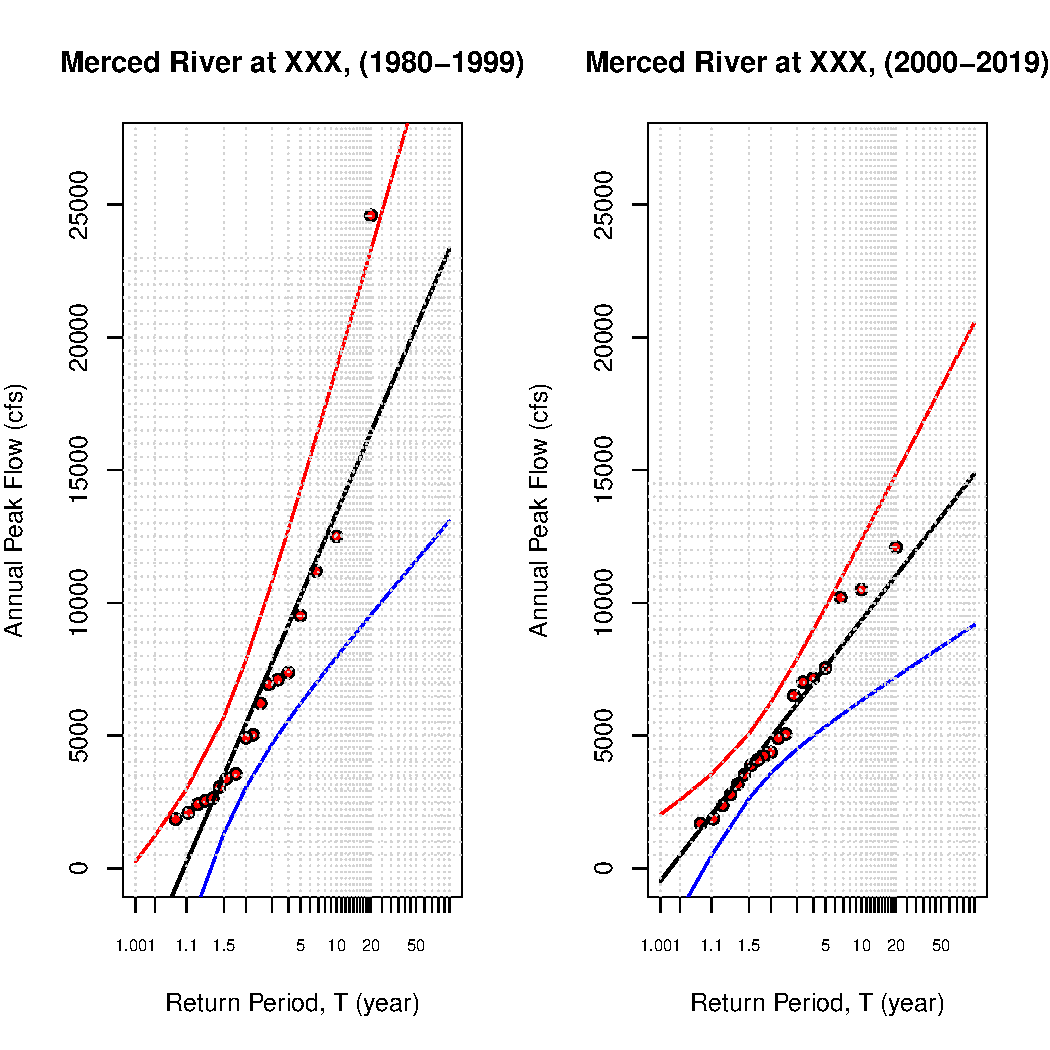
\includegraphics[width=\maxwidth]{figure/unnamed-chunk-7-1} 
\begin{kframe}\begin{alltt}
\hlkwd{par}\hlstd{(}\hlkwc{cex} \hlstd{=} \hlnum{1}\hlstd{)}
\end{alltt}
\end{kframe}
\end{knitrout}

\subsection{Next Steps}

make scales on y-axis the same!

\section{Creating a function}


\end{document}
